\documentclass[12pt]{article}
\usepackage{sbc-template}
\usepackage[utf8]{inputenc}
\usepackage[portuguese]{babel}
\usepackage{lipsum} 
\usepackage{graphicx,url}
\usepackage{amsmath,bm,bbm} 
\usepackage{natbib}
\usepackage[colorlinks=true, allcolors=blue]{hyperref} 
\graphicspath{{../../Images/}}

\sloppy

\title{Caracterização de imagens PolSAR utilizando Bandt-Pompe PDF e Teoria da Informação}

\author{Danilo Fernandes\inst{1}, Eduarda Chagas\inst{2}, , Roger Almeida\inst{1}}


\address{
  Laboratório de Computação Científica e Análise Numérica (LaCCAN)\\
  Universidade Federal de Alagoas (UFAL) -- Maceio, AL -- Brazil
  \nextinstitute
  Departamento de Ciência da Computação\\
  Universidade Federal de Minas Gerais (UFMG) -- Belo Horizonte, MG -- Brazil
  \email{eduardachagas48@laccan.ufal.br}
}

\begin{document}

\maketitle

\section{Processo de simbolização de Bandt-Pompe para padrões bidimensionais}

Para aplicarmos a simbolização de dados bidimensionais seguindo a metodologia proposta por~\cite{PermutationEntropyANaturalComplexityMeasureforTimeSeries2002} devemos considerar, em ambas dimensões, os parâmetros utilizados no algoritmo original. Para fins didáticos, iremos assumir como exemplo uma matriz de tamanho $3$ x $3$, definida a seguir.

\begin{center}
$$
X = \left[
\begin{array}{ccc}
3 & 4 & 8 \\
5 & 6 & 7 \\
2 & 8 & 9 
\end{array}
\right]
$$
\end{center}

O primeiro passo é definir as submatrizes deslizantes e para isso quatro parâmetros são necessários: As dimensões $D_{x}, D_{y} \geq 2$, que são o número de elementos que iram formar os padrões ordinais em ambas dimensões e os delays $\tau _{x}$ e $\tau_{y}$, que informam o quão separados espacialmente estão os símbolos nas duas direções. Neste exemplo, assumiremos $D_{x} = D_{y} = 2$ e $\tau_{x} = \tau_{y} = 1$, obtendo os seguintes quatro particionamentos:

\[
\begin{bmatrix}

A = \left[
\begin{array}{cc}
3 & 4 \\
5 & 6 
\end{array}
\right],

B = \left[
\begin{array}{cc}
4 & 8 \\
6 & 7 
\end{array}
\right],

C = \left[
\begin{array}{cc}
5 & 6 \\
2 & 8 
\end{array}
\right],

D = \left[
\begin{array}{cc}
6 & 7 \\
8 & 9 
\end{array}
\right]

\end{bmatrix}
\]

Após realizar este subdivisão, devemos investigar quais padrões aparecem dentro dos elementos das submatrizes. Para isto, iremos analisar os elementos das destes conjuntos linha por linha, assim $\Pi_{a} = (0,1,2,3)$, pois ao permutar ordenadamente os elementos teremos $a_{1} < a_{2} < a_{3} < a_{4}$. Logo, vamos ter $\Pi_{b} = (0,2,3,1)$, $\Pi_{c} = (2,0,1,3)$ e $\Pi_{d} = (0,1,2,3)$. 

Para todos os padrões ordinais associados a $X$ nós calculamos a distribuição de probabilidade e assim podemos calcular os descritores causais citados anteriormente.

\section{Simulação numérica}

Nossos resultados são baseados em amostras correspondentes à banda HHHH de um conjunto de imagens SAR. Para isso, fizemos um estudo das seguintes regiões capturadas em dados SAR:

\begin{itemize}
    \item Parque Nacional Sierra del Lacandon, Guatemala (adquirido em 10 de abril de 2015), disponível em \url{https://uavsar.jpl.nasa.gov/cgi-bin/product.pl?jobName=Lacand_30202_15043_006_150410_L090_CX_01#dados};
    \item Regiões oceânicas do Cabo Canaveral (adquirido em 22 de setembro de 2016);
    \item Área urbana da cidade de Munique, na Alemanha (adquirido em 5 de junho de 2015).
\end{itemize}

Para aplicar as técnicas aqui definidas, retiramos amostras de dimensão 200x200 e no total utilizamos 20 regiões, assim definidas:  

\begin{itemize}
    \item Quatro regiões florestais da Guatemala;
    \item Uma região de cultivo da Guatemala;
    \item Três regiões terrestres da Guatemala caracterizadas por apresentarem um comportamento não uniforme;
    \item Oito regiões do Cabo de Canaveral, possuindo características de dois comportamentos diferentes;
    \item Quatro regiões urbanas da cidade de Munique.
\end{itemize}

Cada amostra foi redimensionada para um conjunto de matrizes obtidas de partições deslizantes da imagem onde testamos o conjunto de valores $(2,3,4,5,6)$ para as dimensões $D_{x}$ e $D_{y}$ das partições geradas. Para o delay usamos os valores $(1,2,3,4,5)$. O processo de simbolização de Bandt-Pompe é realizado para cada partição, sendo importante salientar que cada dimensão $D_{x}$ e $D_{y}$ leva a $(D_{x}D_{y})!$ possíveis padrões ordinais. 

Enfatizamos que, o uso de rotinas otimizadas implementadas na linguagem \texttt C melhoraram notavelmente o tempo de processamento do experimento, quando comparado com as tradicionais rotinas implementadas anteriormente em \texttt R. Para adquirir a distribuição de probabilidade de Bandt-Pompe é necessário chamar por meio da interface \texttt{.Call()} uma função inteiramente escrita em \texttt C. Esta função em \texttt C recebe como parâmetros uma matriz contendo as amostras já redimensionadas em particionamentos, a quantidade de colunas que a matriz possui, o que equivale à dimensão $D$, e a quantidade de linhas, que representa a quantidade de casos a serem analisados.

Para cada matriz de representação, calculamos duas medidas de complexidade: Entropia de permutação normalizada $H$ e a Complexidade estatística $C$. Em seguida, aplicamos os valores H e C no plano complexidade-entropia que consiste de uma poderosa ferramenta de discriminação e quantificação das diferentes características dos dados.

\section{Resultados e conclusões}

Sabendo que objetivamos caracterizar as diferentes regiões coletadas em dados SAR, realizamos testes com alguns valores de dimensão e delay. Avaliamos a implicação da modificação destes parâmetros no processo de caracterização destes dados no plano Complexidade-Entropia, como podemos verificar abaixo. 

No gráfico gerado com todas as configurações de dimensões e delays, visualmente representamos as diferentes regiões do seguinte modo:

\begin{itemize}
    \item Regiões florestais -- Triângulos cinza; 
    \item Regiões de cultivo -- Triângulos azul escuro;
    \item Regiões não uniforme -- Triângulos violeta;
    \item Regiões oceânicas (Comportamento 1) -- Losangos azul;
    \item Regiões oceânicas (Comportamento 2) -- Losangos verdes;
    \item Regiões urbanas -- Círculos laranjas.
\end{itemize}

Após realizada a caracterização destes dados, algumas questões e pontos despertaram a curiosidade:

\begin{itemize}
    \item Porque os dados parecem seguir um comportamento linear?
    \item Os dados associados a regiões urbanas aparecem muito espaçados em todas as configurações de dimensão e delay. Seria isto um comportamento típico deste tipo de dado? 
    \item Regiões de cultivo e Regiões oceânicas (comportamento 1) deram sinais de que podem se encontrar em áreas semelhantes do plano.
    \item Ao analisar apenas os dados de regiões da Guatemala, a melhor configuração para diferenciar as imagens foram os planos HC ($D = 4$, $\tau = 5$) e ($D = 6$, $\tau = 1$). Entretanto, não podemos concluir que estas configurações se aplicam para as novas amostras estudadas.
    \item Outra característica interessante foi o destaque dos diferentes comportamentos dos dados das regiões oceânicas do Cabo de Canaveral. 
\end{itemize}

Desse modo, desejamos que com a finalização deste trabalho tais questionamentos sejam respondidos.

\begin{figure}[!h]
	\centering
	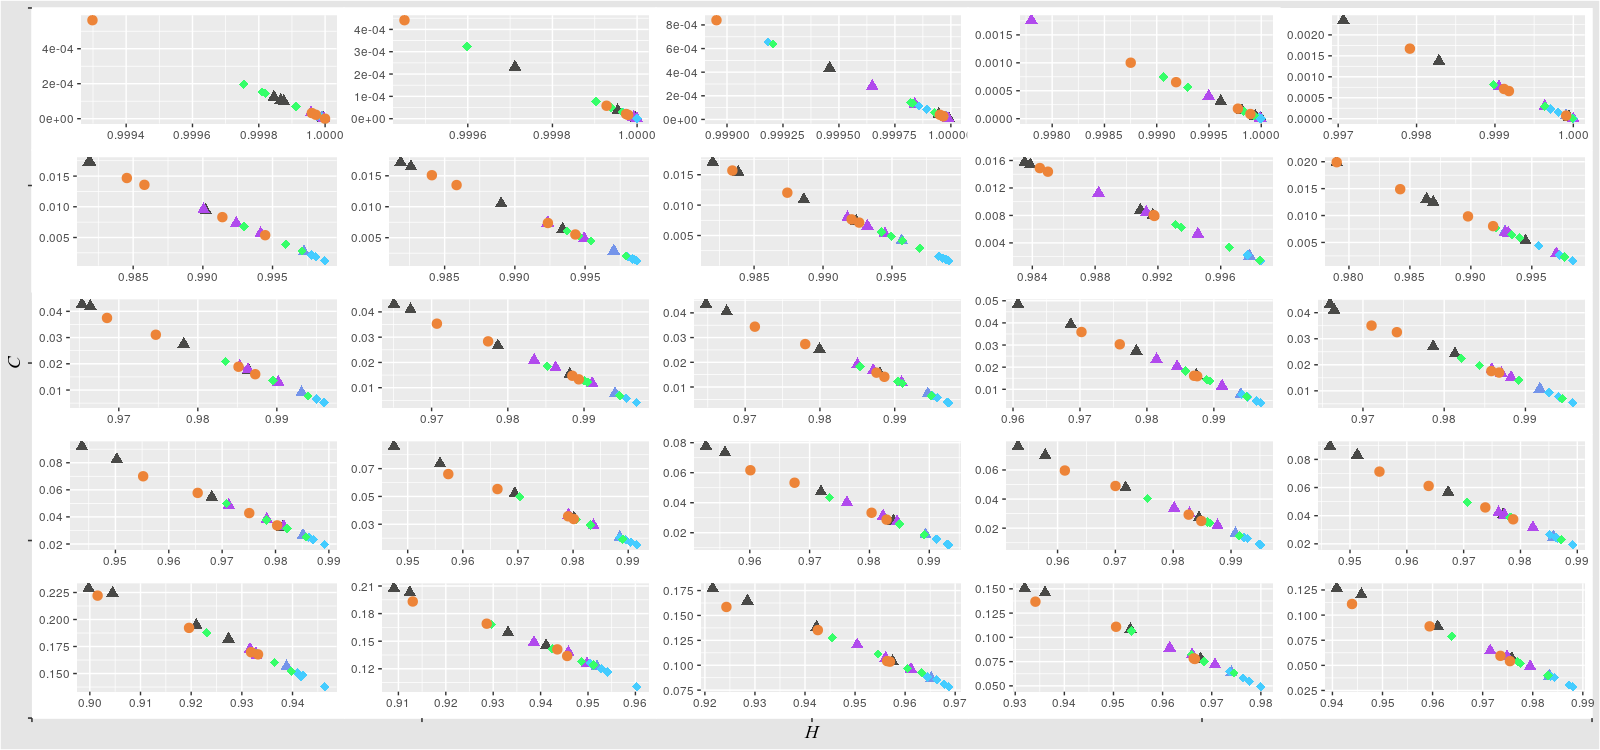
\includegraphics[scale = 0.35]{../../Images/SAR/SAR_regions.png}        
     \caption{Plano Complexidade-Entropia aplicado as amostras correspondentes à banda HHHH de uma imagem SAR. Verticalmente temos as variações dos valores de delay e horizontalmente dos diferentes valores de dimensão aplicados.}
     \label{fig:Plano}
\end{figure}



\bibliographystyle{agsm}
\bibliography{../../Common/references}
\end{document}
